We analyze a combined sample of the two closely related programs: ABC and CARE. Table~\ref{tab:abc-care-characteristics} summarizes their main features. Both interventions were implemented by researchers at the Frank Porter Graham Center (FPG) at the University of North Carolina Chapel Hill, and targeted children from disadvantaged families in the Chapel Hill area. ABC had four cohorts born between 1972 and 1977, and CARE had two cohorts born between 1978 and 1980. Eligibility was determined on the basis of a High Risk Index (HRI) developed for ABC and adapted for CARE \citep{Ramey_Smith_1977_AJMD,Wasik_Ramey_etal_1990_CD}. Components of the HRI include father's presence, parental employment, and participation in welfare.\footnote{See Appendix~\ref{app:eligibility-pop} for the full list of the determinants of HRI \citep{Ramey_Smith_1977_AJMD, Wasik_Ramey_etal_1990_CD, Ramey_Campbell_1991_childreninpoverty}.} Based on these eligibility requirements, \citet{Garcia_Heckman_Leaf_etal_2017_Comp_CBA_Unpublished} calculate that 43\% of African Americans were eligible during the period of intervention and that 19\% of all African American children are eligible now.

Both interventions involved intensive center-based care for subjects in the treatment group starting at 8 weeks and continuing until age 5 before the children started kindergarten. In addition to free access to this center-based care, treatment-group subjects also received daily health screenings, diapers, and formula for 6 months. Control-group families received diapers and formula as well for the same period of time.\footnote{\citet{Wasik_Ramey_etal_1990_CD,Ramey_Campbell_1991_childreninpoverty}.} Between ages 5 and 8, there was an additional component of treatment with home visits to tutor the children and to encourage families to be involved in their child's schooling. In CARE, all the subjects who received center-based care also received this school-age component. In ABC, treatment status of this component was randomized. We do not analyze the post-5 home-based visits because previous work has found that this component of treatment has no statistically significant impact \citep{Campbell_Ramey_etal_2002_ADS,Campbell_Conti_etal_2014_EarlyChildhoodInvestments}.

\begin{table}[!htbp]
\centering
\caption{Overview of the ABC and CARE Programs}
\label{tab:abc-care-characteristics}
\begin{threeparttable}
	\begin{tabular}{l l}
	\toprule
Site & Chapel Hill, North Carolina \\
Cohorts & 4 (ABC), 2 (CARE) \\
$N$ & 58 treatment, 56 control (ABC) \\
	& 17 treatment, 23 control (CARE) \\
\midrule
Eligibility & HRI $>$ 11 \\
		& Biologically healthy \\
\midrule
Treatment years & 1972--1981 (ABC), 1977--1985 (CARE) \\
Treatment duration & 5 years \\
\midrule
Home visits 	& 2.5--2.7	per month (CARE)	\\
Center care	& 50	weeks per year \\
		 	& 30--45 hours per week  \\
Other treatment components & Formula until 6 months\\
					& Diapers until 6 months \\ 
					& Health check-ups \\
					& Medical care \\
					& Parenting instruction \\
					& Counseling \\
					& Transportation to center \\
Control-group incentives & Formula until 6 months \\
				& Diapers until 6 months 	\\
				& Health check-ups until 1 year (ABC, cohort 1) \\
\midrule
Adult-child ratio & 1:3--1:6 \\
Teacher requirements & High school through masters \\
				& Experience with kids \\
Specialists & Physician, nurse, social worker \\
\bottomrule
\end{tabular}



\begin{tablenotes}
\footnotesize
\item \textbf{Note:} Biologically healthy includes lack of serious illness, including mental retardation. \\
\item \textbf{Sources:} \citet{Ramey_Collier_etal_1976_CarolinaAbecedarianProject,Ramey_Smith_1977_AJMD,Ramey_etal_1985_Project-CARE_TiECSE,Wasik_Ramey_etal_1990_CD,Ramey_Campbell_1991_childreninpoverty}.
\end{tablenotes}
\end{threeparttable}
\end{table}

The program focused on developing language, cognition, and social-emotional skills.\footnote{During ABC and CARE, the \textit{Learning Games} curriculum was developed and refined \citep{Sparling_Lewis_1979_BOOKLearninggamesFirstThree,Sparling_Lewis_1984_BOOKLearningGamesThreesFours}.} Program curricula emphasized child-led learning of skills important for future learning \citep{Ramey_Smith_1977_AJMD, Wasik_Ramey_etal_1990_CD, Ramey_Campbell_1991_childreninpoverty}. The teachers and classroom aids were trained throughout the intervention. Researchers and child development experts at FPG observed classroom interactions and gave detailed feedback to the instructors \citep{Ramey-etal_2012-ABC}.\footnote{These aspects of the program relate to structural quality rather than process quality, i.e., the daily experiences of the children \citep{Thomason_LaParo_2009_EED}. Aspects of structural quality, including low child-teacher ratios, small group sizes, and teacher education, are often associated with high process quality \citep{Phillipsen_etal_1997_ECRQ}. However, recent studies find that curricula and professional development are even more highly correlated with process quality. This is especially true if the curricula and professional development are informed by knowledge of child development \citep{Slot_etal_2015_Dutch_ECRQ}. Although measures of process quality (e.g., measures of teacher-child interactions) are not available for the ABC/CARE subjects, the curricula and professional development offerings were intensive, especially compared to standards of that era \citep{Burchinal_etal_1989_CD_Daycare-Pre-K-Dev}.}

CARE included an additional arm of treatment. Besides the services offered in ABC, those in the CARE treatment group also received home visiting from birth to age 5. Home visiting consisted of biweekly visits focusing on improving parental problem-solving skills. To test the effectiveness of this home-visiting component, there was a third randomized group ($N=23$) that received only the home visiting component at ages 0-5, but not center-based care \citep{Wasik_Ramey_etal_1990_CD}. In light of previous analyses of CARE finding no effect of the early-age home-visiting component, we drop this last group from our analysis.\footnote{\citet{Campbell_Conti_etal_2014_EarlyChildhoodInvestments} and \citet{Burchinal_etal_2006_MSRCD_IV-Growth-Curve} test and do not reject the hypothesis of no treatment effects for this additional component of CARE.} These analyses justify merging the treatment groups of ABC and CARE. We henceforth analyze the samples as coming from a single ABC/CARE program.

Table~\ref{tab:abccare-baseline} compares pre-program variables for experimental and gender groups. The only marginally statistically significant difference in baseline variables between boys and girls is in the HRI score, which is 1.78 points lower for males than for females, consistent with their better home environments. A higher HRI is associated with greater disadvantage.

\begin{table}[!htbp]
\centering
\caption{Baseline Differences, ABC/CARE}
\label{tab:abccare-baseline}
\begin{threeparttable}
	\begin{tabular}{l c c c c c c}
\toprule
\mc{1}{c}{Variable} & Female & Male & $ p $ -value & Control & Treatment & $ p $ -value \\
& Mean & Differential & & Mean & Differential & \\
\midrule
Mother's age &                19.72 &                 1.13 &                 0.15 &                20.52 &                -0.51 &                 0.51 \\
Mother works &                 0.23 &                 0.09 &                 0.28 &                 0.21 &                 0.11 &                 0.18 \\
Mother's IQ &                84.46 &                 1.33 &                 0.46 &                84.65 &                 0.98 &                 0.58 \\
Father at home &                 0.24 &                 0.04 &                 0.56 &                 0.29 &                -0.05 &                 0.51 \\
Number of siblings &                 0.59 &                 0.07 &                 0.67 &                 0.71 &                -0.18 &                 0.29 \\
HRI score &                21.57 &                -1.78 &                 0.06 &                21.39 &                -1.47 &                 0.13 \\
Apgar score, 1 min. &                 7.68 &                -0.07 &                 0.80 &                 7.60 &                 0.09 &                 0.76 \\
Apgar score, 5 min. &                 8.94 &                -0.20 &                 0.33 &                 8.87 &                -0.04 &                 0.83 \\
Birthweight &                 7.18 &                -0.20 &                 0.34 &                 7.17 &                -0.19 &                 0.38 \\
Gestational age &                39.85 &                -0.42 &                 0.27 &                39.87 &                -0.50 &                 0.19 \\
\bottomrule
\end{tabular}
% This file generated by: /scripts/abccare/treatment-effects/abccare-baseline.do

\begin{tablenotes}
\footnotesize
\item \textbf{Note:} The variables in this table are all measured at baseline, close to when the children were born. Maternal labor supply (``Mother works'') is represented using an indicator variable. A larger HRI (High Risk Index) score indicates more disadvantage. Apgar, measured at 1 and 5 minutes after birth, is a test of the health condition of newborn babies. A score closer to 10 indicates a healthier condition \citep{Apgar_1966_APGAR-Scoring_PCNA}. Birthweight is in pounds and gestational age is in weeks. Control means and treatment differentials pool males and females.
\end{tablenotes}
\end{threeparttable}
\end{table}

\subsection{The Randomization Protocol} \label{section:randomization}

Randomization for ABC/CARE was conducted on child pairs matched on family background. Siblings and twins were jointly randomized into either treatment or control groups. For siblings, this only occurred when two siblings were close enough in age so that both of them were eligible for the program. Pairing was based on the High Risk Index, as well as maternal education, maternal age, and gender of the subject.\footnote{We do not know the original pairs.}

ABC collected an initial sample of 121 subjects. All providers of health care and social services (referral agencies) in the area of the ABC/CARE study were informed of the programs. They referred mothers whom they considered disadvantaged. Eligibility was corroborated before randomization. Encouragement from the referral agencies was such that all but one of the referred mothers agreed to participate in the initial randomization.\footnote{\citet{Ramey_Yeates_Short_1984_CD,Campbell_Ramey_1995_AERJ}.}  We discuss the pattern of missing observations in Appendix~\ref{appendix:randomization}. In Appendix~\ref{appendix:estimates}, we document that our estimates are robust when we adjust for missing data using standard weighting methods described in Appendix~\ref{app:method_partialobs}.

Twenty-two subjects in ABC did not stay in the program through age 5. The number of dropouts is evenly balanced across treatments and controls. Dropping out was primarily related to the health of the child and the mobility of families rather than as a result of  dissatisfaction with the program. The 22 dropouts include four children who died, four children who left the study because their parents moved, and two children who were diagnosed as developmentally delayed.\footnote{\citet{Burchinal_Campbell_etal_1997_CD}.} Details are in Table~\ref{table:abccompromises}. Everyone offered the program was randomized to either treatment or control. Dropping out occurs \emph{after} randomization and is balanced across treatment groups. We conduct the same analysis for the CARE sample, although there were far fewer dropouts and there was no compromised randomization.\footnote{The modest sample size after accounting for dropouts, especially after dividing the sample by male and female, is unavoidable. No datasets have the experimental design and longitudinal data collection of ABC/CARE with a large sample. Future research should repeat these analyses in larger studies (e.g., the Infant Health and Development Program) as the subjects continue to age.}

\subsection{Control Group Substitution}

In ABC/CARE, many control-group subjects (but no treatment-group subjects) attended alternative center-based care.\footnote{See \cite{Heckman_Hohmann_etal_2000_QJE} and \citet{Kline_Walters_2016_QJE} on the issue of substitution bias in social experiments.} The figure is \treatsubsabc\ for ABC and \treatsubscarec\ for CARE. This information comes from a survey administered to ABC/CARE families asking about the childcare arrangements made during each month between birth and age 5. Home care includes parental care, but also care of a relative, neighbor, or friend. The survey also captured specifics, such as the name of the center-based institutions, allowing for a detailed understanding of alternative care environments.

\begin{sidewaysfigure}[!htbp]
\centering
\caption{Control Substitution Characteristics, ABC/CARE Control Group}\label{fig:control-sub}
\begin{subfigure}[h]{0.49\textwidth}
	\centering
	\caption{Cumulative Enrollment} \label{fig:treatsubcare}
	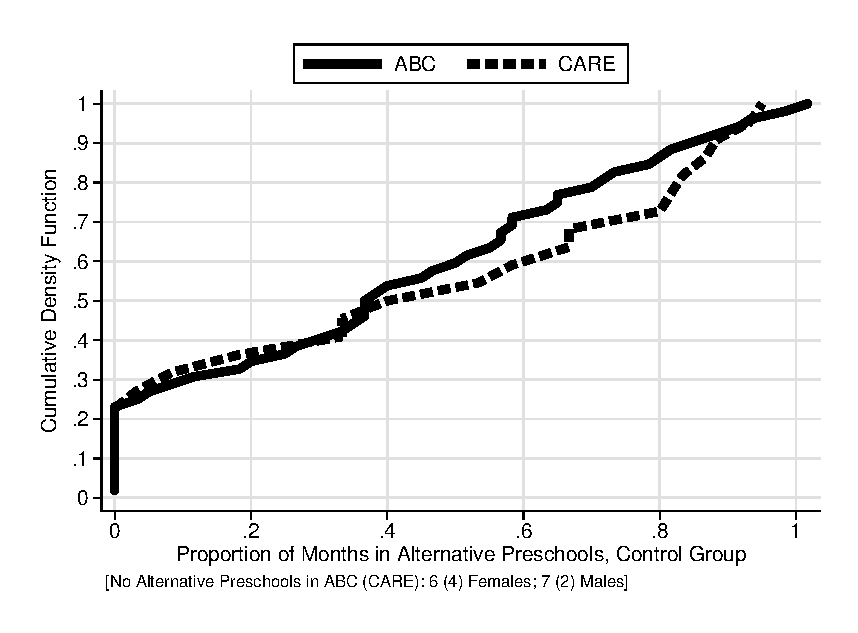
\includegraphics[width=\textwidth]{output/abccare_controlcontamination.eps}
\end{subfigure}
\begin{subfigure}[h]{0.49\textwidth}
	\centering
	\caption{Enrollment Dynamics} \label{fig:proportion-alt-pre}
	\includegraphics[width=\textwidth]{output/abccare_Vprobs.eps}
\end{subfigure}%
\footnotesize \justify
Note: Panel (a) displays the cumulative distribution function of enrollment in alternatives. Panel (b) displays the fraction of ABC/CARE control-group children enrolled in alternatives, conditional on being enrolled in the previous age (at least one month).\\
\end{sidewaysfigure}

Figure~\ref{fig:treatsubcare} shows the cumulative distribution of the proportion of time in the first five years that control subjects were enrolled in alternative formal childcare programs. Figure~\ref{fig:proportion-alt-pre} shows the dynamics of enrollment. Those who enrolled generally stay enrolled over time. As control-group children aged, they were more likely to enter childcare.\footnote{See Figure~\ref{fig:control-sub_a} in Appendix~\ref{app:control-subbb}.}

As a group, the children in the control group that enrolled in alternative early childcare programs are less economically disadvantaged at baseline compared to children who stay at home, although, as we show below, there are important differences by gender of the child. Disadvantage is measured by maternal education, maternal IQ, Apgar scores, and the High Risk Index that defines ABC/CARE eligibility. Control children who attend alternative formal care generally have fewer siblings. On average, they are children of mothers who are more likely to be working at baseline (statistically significant at 10\%). Parents of girls are much more likely to use alternative center childcare if assigned to the control group.

Table~\ref{table:controlsubscharacteristics} tests differences across these variables between children in the control group who attended and those who did not attend alternative childcare. The only statistically significant difference in observed baseline characteristics between the controls who use formal childcare and those who stay at home is whether the mother works. The mother is more likely to work at baseline for children attending alternative care. We discuss selection into alternative care settings by gender of the child in Section~\ref{sec:gender-differences}.

While most of the alternative childcare centers received federal subsidies and were subject to the federal regulations of the era, they were relatively low-quality compared to ABC/CARE \citep{Burchinal_etal_1989_CD_Daycare-Pre-K-Dev}. In terms of child-staff ratios, ABC/CARE far exceeded the highest state and federal standards of the day.\footnote{Appendix~\ref{appendix:tetanus} shows this and discusses the standards of the day \citep{Department-of-Health_1968_DayCareRequirements,NCGA_1971_House-Bill-100,Ramey-et-al_1977_Intro-to-ABC,Ramey_Campbell_1979_SR,Ramey_McGinness_etal_1982_Abecedarianapproach,Burchinal_Campbell_etal_1997_CD}} We do not have baseline information on the quality of the parent-child interaction to be able to precisely analyze the environments of those who stayed at home.

When we compare ABC/CARE treatment to that from alternative preschools, ABC/CARE produces substantial treatment effects. Parents perceived that ABC/CARE was superior to alternative preschools because all offered it chose to participate in it. The access of control-group children to alternative programs creates both a problem of substitution bias and an opportunity to learn about the benefits or harms of lower-quality childcare arrangements. Exploiting the heterogeneous experiences of the control-group subjects, we isolate the effects of developmentally enriched environments compared to home environments, and the effects of  lower-quality center environments compared to home environments for boys and girls.

\subsection{Data Collection}

Measures of cognitive, social-emotional, and parenting skills were collected during the intervention and while the subjects were in school.\footnote{Time-use data are not available.} The researchers collected information on the subjects' academic performance including grade retention and special education. The adult surveys (at ages 21 and 30) cover items related to employment, post-secondary education, health, criminal activity, and family structure. When the subjects were in their mid 30s, the researchers collected administrative crime data and conducted a full medical survey. Appendix~\ref{appendix:results} describes the data that we use more completely.


